\chapter{Как устроена модель SVD-SNO v2}
\label{code:implementation}

Для одного примера известны два узловых поля материала $A,n\in\R^N$,
угол $\theta$ и волновое число $k$. Требуется восстановить комплексное
поле $u_s\in\C^N$ в тех же узлах. Эталонные поля даёт расчёт методом
конечных элементов. В репозитории объект \texttt{Predictor} сначала
кодирует входные данные, вызывает коэффициентную сеть \texttt{SVDSNO},
затем восстанавливает поле. Рассмотрим версию архитектуры~2.

\section{Представление данных и выбор ранга}
\label{code:preprocessing}

По обучающей выборке строят четыре вещественных базиса для $A$, $n$,
$u_R=\operatorname{Re}u_s$ и $u_I=\operatorname{Im}u_s$.
Для каждого поля $v$ сохраняют его среднее $\mu_v\in\R^N$ и матрицу
мод $\Phi_v\in\R^{N\times r_v}$, где $r_v$ --- число оставленных мод.
Для входных базисов берут по одному снимку каждой обучающей среды,
чтобы число запросов к среде не определяло её вес в POD. Для выходных
базисов берут все обучающие поля рассеяния. Диагональную матрицу узловых
весов $W=\diag(M\bm 1)$ получают из сумм строк согласованной матрицы
масс $M$. В этой метрике имеем
\begin{equation}
 \Phi_v^\top W\Phi_v=I,\qquad
 c_v=\Phi_v^\top W(v-\mu_v),\qquad
 v_r=\mu_v+\Phi_v c_v .
 \label{code:pod-encoding}
\end{equation}
Если все обучающие среды одинаковы, центрированные входные снимки
нулевые и оба входных ранга равны нулю. Сами $A,n$ при этом могут
существенно меняться от узла к узлу.

Длину выходной таблицы $r_{\rm out}$ выбирают по валидационной выборке
$V$. Кандидаты $r$ идут от 1 до максимального доступного ранга двух
выходных базисов. В каждой компоненте используют первые $r$ мод или
весь базис, если его ранг меньше. Коэффициенты находят по формуле
\eqref{code:pod-encoding} с весами $W$, а комплексную реконструкцию
$u^{(t)}_{s,r}$ оценивают в норме $M$:
\begin{equation}
 E_V(r)=\frac{1}{|V|}\sum_{t\in V}
 \frac{\norm{u_s^{(t)}-u^{(t)}_{s,r}}_M}{\norm{u_s^{(t)}}_M},
 \qquad \norm{v}_M^2=v^*Mv .
 \label{code:rank-criterion}
\end{equation}
Выбирают первый ранг, при котором средняя ошибка не превышает
заданного порога. Если порог недостижим, оставляют наибольший доступный
ранг и сохраняют признак этого случая. У вещественного и мнимого
базисов итоговые ранги $r_R,r_I$ могут различаться. Для более короткого
базиса недостающие столбцы при восстановлении поля считаются нулевыми.
Критерий~\eqref{code:rank-criterion} характеризует точность представления
на валидации, до обучения коэффициентной сети.

\section{Из входных признаков в коэффициенты поля}
\label{code:network}

Входные POD-коэффициенты и волновое число нормируют с помощью средних
и стандартных отклонений обучающей выборки. Каждый признак $x$
преобразуют по правилу $\widetilde x=(x-m)/s$, где $m$ и $s$ ---
среднее и стандартное отклонение значений этого признака по обучающим
примерам. Для почти постоянного признака код принимает $s=1$.
Вектор признаков одной задачи равен
\begin{equation}
 f=(\widetilde c_A,\widetilde c_n,\cos\theta,\sin\theta,\widetilde k)
       \in\R^{r_A+r_n+3}.
 \label{code:feature-vector}
\end{equation}
Функция \path{coefficient_tokens} превращает его в таблицу из
$R=\max(r_A,r_n,r_{\rm out})$ строк и пяти столбцов:
\begin{equation}
 T_{j,:}=(a_j,\eta_j,\cos\theta,\sin\theta,\widetilde k),\qquad
 1\le j\le R .
 \label{code:tokens}
\end{equation}
Последовательность $a$ содержит $\widetilde c_A$ и затем нули до
длины~$R$. Так же, независимо, дополняют $\widetilde c_n$, получая $\eta_j$.
Индекс строки $j$ указывает позицию в каждой последовательности.
Базисные функции, стоящие на этой позиции у $A$ и $n$, могут различаться.
Угловые признаки сохраняют периодичность $\theta$ и доступны каждой строке.
Например, при $r_A=3$, $r_n=1$ и $r_{\rm out}=2$ получаем $R=3$.
В первые два столбца записывают
$a=(\widetilde c_{A,1},\widetilde c_{A,2},\widetilde c_{A,3})^\top$
и $\eta=(\widetilde c_{n,1},0,0)^\top$. Третий коэффициент $A$
может влиять на первые две строки через смешивание модальных позиций.

Каждую строку переводят из пяти чисел в $H$ скрытых признаков:
$Z_0=\GELU(TW_0+\bm 1 b_0^\top)$, где $W_0\in\R^{5\times H}$,
$b_0\in\R^H$, а $\bm 1$ --- столбец из $R$ единиц.
Здесь и далее $\GELU(t)=t\,\mathbb P(\xi\le t)$ для
$\xi\sim\mathcal N(0,1)$ действует поэлементно. Далее сеть применяет
$L$ блоков с разными наборами весов. Для одного блока имеем
\begin{equation}
 Z^+=Z+\GELU\bigl(ZW_{\rm loc}+\bm 1 b^\top+BZ W_{\rm ch}\bigr),
 \qquad Z,Z^+\in\R^{R\times H}.
 \label{code:block}
\end{equation}
Матрицы $W_{\rm loc},W_{\rm ch}\in\R^{H\times H}$ действуют справа на
каналы. Матрица $B\in\R^{R\times R}$ действует слева на модальные
позиции. Первая ветвь преобразует каждую строку отдельно. Во второй
ветви результат для позиции $j$ зависит от других строк через $B_{ji}$.
Слагаемое $Z$ переносит исходную таблицу в следующий слой
(рис.~\ref{code:block-diagram}).
В PyTorch матрица слоя \texttt{Linear} действует по последней оси,
поэтому для применения $B$ код временно меняет местами оси строк и каналов.

\begin{figure}[htbp]
\centering
\begin{tikzpicture}[
  stage/.style={draw=teal,fill=soft,rounded corners=2pt,align=center,
                minimum height=7mm,inner xsep=2.5mm,font=\small},
  sum/.style={circle,draw=teal,fill=soft,inner sep=1pt,minimum size=5mm},
  wire/.style={-{Stealth[length=2mm]},semithick,draw=navy},
  route/.style={semithick,draw=navy}]
  \node (z) at (0,0) {$Z$};
  \node[stage] (local) at (3,0.66) {$ZW_{\rm loc}+\bm 1b^\top$};
  \node[stage] (mixed) at (3,-0.66) {$B(ZW_{\rm ch})$};
  \node[sum] (sum) at (5.25,0) {$+$};
  \node[stage] (gelu) at (6.7,0) {$\GELU$};
  \node[sum] (add) at (8.25,0) {$+$};
  \node (out) at (9.5,0) {$Z^+$};
  \coordinate (skip) at (0.75,0);
  \coordinate (split) at (1.40,0);
  \coordinate (merge) at (4.65,0);
  \draw[route] (z) -- (split);
  \fill[navy] (skip) circle (1.4pt);
  \fill[navy] (split) circle (1.4pt);
  \draw[wire] (split) |- (local.west);
  \draw[wire] (split) |- (mixed.west);
  \draw[wire] (local.east) -| (merge) -- (sum.west);
  \draw[route] (mixed.east) -| (merge);
  \draw[wire] (sum) -- (gelu);
  \draw[wire] (gelu) -- (add);
  \draw[wire] (skip) -- (0.75,-1.35) -- (8.25,-1.35) -- (add.south);
  \draw[wire] (add) -- (out);
  \node[font=\small\sffamily,text=navy,below] at (4.5,-1.35) {Остаточная связь};
\end{tikzpicture}
\caption{Две ветви блока сначала суммируются. После GELU к результату
прибавляется входная таблица. Размер каждой таблицы равен $R\times H$.}
\label{code:block-diagram}
\end{figure}

Общее для строк аффинное отображение $H\to 2$ применяется к первым
$r_{\rm out}$ строкам $Z_L$. В строке $j$ оно вычисляет
$\widehat q_{j,:}=(Z_L)_{j,:}W_{\rm out}+b_{\rm out}^\top$, где
$W_{\rm out}\in\R^{H\times 2}$ и $b_{\rm out}\in\R^2$.
Два столбца $\widehat q_{j,\alpha}$, $\alpha\in\{R,I\}$, задают
коэффициенты в нормированных единицах.
Для каждой моды и компоненты хранятся отдельные среднее $m_{j,\alpha}$
и масштаб $s_{j,\alpha}$. Декодер вычисляет
\begin{align}
 \widehat c_{j,\alpha}&=m_{j,\alpha}+s_{j,\alpha}\widehat q_{j,\alpha},
                         \label{code:denormalize}\\
 \widehat u_\alpha&=\mu_\alpha+\Phi_\alpha\widehat c_\alpha,
 \qquad \widehat u_s=\widehat u_R+\ii\widehat u_I .
                         \label{code:decode-physical}
\end{align}
В произведении на $\Phi_\alpha$ участвуют только $r_\alpha$ активных
коэффициентов. Каждая из двух сумм использует собственные моды и среднее.

\section{Как считать ошибку поля по коэффициентам}
\label{code:fem-loss}

При обучении важна величина $\norm{\widehat u_s-u_s}_M$. Прямой расчёт
требовал бы восстанавливать $N$ узловых значений для каждого примера
на каждом шаге. Ту же величину можно получить из квадратичных форм
порядка $r_R$ и $r_I$ и заранее вычисленных остатков двух компонент.

Для одной вещественной компоненты положим $y=u-\mu$,
$G=\Phi^\top M\Phi$. При линейно независимых активных столбцах
$\Phi$ матрица $G$ положительно определена, поскольку
$v^\top Gv=\norm{\Phi v}_M^2>0$ при $v\ne0$. Для наилучшей проекции
минимизируем $\norm{y-\Phi c}_M^2$ по $c$. Приравнивая производную
к нулю, получаем уравнение для $c_*$ и определяем остаток $\rho$:
\begin{equation}
 G c_* =\Phi^\top M y,\qquad \rho=y-\Phi c_* .
 \label{code:consistent-projection}
\end{equation}
Из нормальных уравнений следует $\Phi^\top M\rho=0$. Запишем ошибку
в виде $\widehat u-u=\Phi(\widehat c-c_*)-\rho$ и раскроем квадрат.
Смешанное слагаемое исчезает в силу ортогональности. Получается
\begin{equation}
 \norm{\widehat u-u}_M^2
   =(\widehat c-c_*)^\top G(\widehat c-c_*)+\norm{\rho}_M^2 .
 \label{code:quadratic-identity}
\end{equation}
Первое слагаемое обращается в нуль при точном прогнозе оптимальных
коэффициентов. Второе даёт наименьший достижимый квадрат нормы ошибки
для данного примера и базиса. При нулевом ранге остаётся только ошибка
относительно среднего поля. Формула~\eqref{code:pod-encoding} даёт
коэффициенты проекции с диагональным весом $W$, тогда как $c_*$ и $G$
определяются скалярными произведениями в метрике $M$.

Матрица $M$ вещественна и симметрична, поэтому квадрат комплексной
нормы равен сумме квадратов норм двух компонент. Для примера $t$
обозначим через $e_t$ сумму правых частей~\eqref{code:quadratic-identity}
по $R,I$, а через $d_t=\norm{u_s^{(t)}}_M^2$ --- энергию эталона.
При положительных энергиях обычного масштаба функция потерь в группе
$J$ примеров равна $|J|^{-1}\sum_{t\in J}\sqrt{e_t/d_t}$.
Вблизи нуля реализация использует
\begin{equation}
 \mathcal L_J=\frac1{|J|}\sum_{t\in J}
 \frac{e_t}{\sqrt{\max(e_t,\varepsilon)}\sqrt{\max(d_t,\varepsilon)}},
 \qquad \varepsilon=10^{-24},\quad e_t\ge0 .
 \label{code:stable-loss}
\end{equation}
Энергии остатка вычисляют непосредственно по $\rho$, чтобы избежать
потери точности при вычитании близких энергий. Величины $c_*$,
$\norm{\rho}_M^2$, $d_t$ и обе матрицы $G$ готовят до оптимизации.
Их вычисляют в \texttt{float64} по модам, средним и эталонным полям,
округлённым до \texttt{float32}.
На шаге обучения нужны только предсказанные коэффициенты и сохранённые
величины для примеров этой группы.

\section{Что подбирает процедура обучения}
\label{code:training}

POD-моды, средние и масштабы после подготовки зафиксированы.
На каждом шаге алгоритм AdamW обновляет веса и смещения сети по
градиенту~\eqref{code:stable-loss} на группе обучающих примеров.
Один проход по обучающей выборке называется эпохой. После каждой эпохи
измеряют среднюю ошибку на валидационной выборке. Если она перестаёт
уменьшаться на заданное число эпох, обучение может остановиться раньше.
После обучения возвращают веса эпохи с наименьшей валидационной
ошибкой. Тестовую выборку используют для итоговой оценки этих весов.

\begin{center}
\begin{tabularx}{\linewidth}{@{}l X@{}}
\toprule
Операция & Реализация в каталоге \path{neural_operator/}\\\midrule
Вычисление базиса и проекции & \path{sno/basis.py}, класс \texttt{PODBasis}\\
Строки, входной и выходной слои & \path{sno/model.py}, класс \texttt{SVDSNO}\\
Блок из двух ветвей & \path{_layers.py}, класс \texttt{CoefficientBlock}\\
Квадратичная форма ошибки & \path{losses.py}, класс \texttt{PODFEMLoss}\\
Подготовка и прогноз & \path{training.py}, функция \path{_svd_preprocessing} и класс \texttt{Predictor}\\\bottomrule
\end{tabularx}
\end{center}
Для опыта на эталонной сетке цикл обучения находится в
\path{experiments/reference_sno_gmsfem/training.py}. Шаг AdamW
снижается при остановке улучшения ошибки на валидации.


\clearpage
\section{Что представляют собой матрицы в операторной записи}
\label{code:operator}
Начнём с двух способов ответить на один запрос $p=(A,n,k,\theta)$.
При обратимой дискретной системе оператор решения МКЭ имеет вид
\[
 \mathcal S_h(p)=L_h(A,n,k)^{-1}F(p),\qquad
 L_h=K-k^2 M_n-\ii k B_\Gamma .
\]
Столбец $j$ матрицы $L_h$ показывает действие дискретного уравнения на
узловую функцию $\varphi_j$. Например, $(M_n)_{ij}$ получается
интегрированием $n\varphi_i\varphi_j$ по области, а $(B_\Gamma)_{ij}$~---
интегрированием $\varphi_i\varphi_j$ по внешней границе.
Матрицы собираются из геометрии и свойств среды по~\eqref{math:fem-system}.
Обозначение $L_h^{-1}F$ означает решение системы с правой частью $F$.

У SVD-SNO тот же физический вход и тот же формат выхода. Оператор прогноза
составлен из последовательных отображений:
\begin{equation}
 \widehat{\mathcal S}_h(p)=
 \bigl(\mathcal D\circ\mathcal Q\circ\mathcal F_6\circ\cdots
       \circ\mathcal F_1\circ\mathcal L\circ\mathcal E\bigr)(p).
 \label{code:whole-operator}
\end{equation}
Прочитайте формулу справа налево. Размеры ниже относятся к одному запросу
на эталонной сетке, без оси примеров.

\begin{center}
\renewcommand{\arraystretch}{1.17}
\begin{tabularx}{\linewidth}{@{}l l X@{}}
\toprule
Шаг & Выход & Как получен результат \\ \midrule
$\mathcal E$ & $25\times5$ & Представление запроса по~\eqref{code:tokens}.
Для одной среды материальные коэффициенты отсутствуют, обе первые колонки нулевые.\\
$\mathcal L$ & $25\times48$ & Умножение каждой строки на $W_0$ размера $5\times48$,
сдвиг и GELU. К каждой позиции моды применены одни и те же веса.\\
$\mathcal F_1,\ldots,\mathcal F_6$ & $25\times48$ & Шесть преобразований
вида~\eqref{code:block}. В каждом блоке свой набор весов.\\
$\mathcal Q$ & $25\times2$ & Матрица $W_{\rm out}$ размера $48\times2$ и смещение
переводят строку в два нормированных выходных коэффициента.\\
$\mathcal D$ & $53\,246$ комплексных чисел & Отмена нормировки и две суммы
по модам, одна для каждой компоненты, по~\eqref{code:decode-physical}.\\
\bottomrule
\end{tabularx}
\end{center}

Таблица $Z$ внутри сети имеет 25 строк и 48 столбцов. Строка обозначает
позицию в последовательности мод, столбец~--- скрытый канал, то есть один
из признаков, которые сеть формирует при обучении. Физический смысл двум числам в выходной строке придаёт декодер: после отмены
нормировки первый коэффициент умножает моду $\phi_{j,R}$, второй~---
свою моду $\phi_{j,I}$. В опыте \texttt{low} среда фиксирована,
так что между запросами меняются только $k$ и $\theta$.

\begin{idea}{Какие матрицы меняются при обучении}
$K,M_n,B_\Gamma$ задаёт краевая задача. Матрица $M$ определяет норму
ошибки, а $W$ используется для построения базиса. Матрицы
$U,\Sigma,V$ из~\eqref{math:svd} описывают данные: в точном разложении
$U_{sj}\sigma_j$~--- коэффициент снимка $s$ в моде $j$, а
$W^{-1/2}V_{:,j}$~--- сама пространственная мода.
Оптимизатор меняет $W_0,B_\ell,W_{\rm loc},W_{\rm ch},W_{\rm out}$
и смещения. Пространственные моды остаются зафиксированными.
\end{idea}

\clearpage
\subsection{Один вес, один элемент таблицы}
\label{code:matrix-entries}
Рассмотрим линейную часть одного блока до добавления смещения и GELU.
Через $\mathcal A_\ell$ обозначим оператор на таблицах $Z$:
\[
 \mathcal A_\ell(Z)=ZW_{\rm loc}+B_\ell ZW_{\rm ch}.
\]
В обеих ветвях веса каналов имеют размер $48\times48$.
$W_{\rm loc}$ смешивает каналы в пределах одной строки. $W_{\rm ch}$
смешивает каналы глобальной ветви, а $B_\ell$ размера $25\times25$
передаёт результат между строками. Как узнать, куда попадёт одна запись?
Пусть $E_{ja}$~--- таблица с единицей на месте «мода $j$, канал $a$» и
нулями в остальных ячейках. В позиции «мода $i$, канал $b$» получим
\begin{equation}
 [\mathcal A_\ell(E_{ja})]_{ib}
 = \delta_{ij}(W_{\rm loc})_{ab}+(B_\ell)_{ij}(W_{\rm ch})_{ab}.
 \label{code:impulse}
\end{equation}
Здесь $\delta_{ij}=1$ при $i=j$ и равна нулю при $i\ne j$.
Столбец $j$ матрицы $B_\ell$ задаёт, с какими весами исходная позиция $j$
действует на все выходные позиции $i$. Строка $a$ матрицы $W_{\rm ch}$
определяет передачу исходного канала $a$ во все выходные каналы $b$.

\begin{worked}{Проверка на весах обученной модели}
Прибавим к входу первого блока $E_{2,1}$ и посмотрим изменение первой
строки в первом канале \emph{до активации}. Из сохранённых весов
$(B_1)_{1,2}=-0{,}082126$, $(W_{\rm ch})_{1,1}=-0{,}076866$.
Поскольку $1\ne2$, вклад локальной ветви равен нулю. Глобальная
ветвь даёт $(-0{,}082126)(-0{,}076866)\approx0{,}006313$.
Это передача между двумя модальными позициями, измеренная в скрытом канале.
Узловое поле появится только после выходного слоя и декодирования.
\end{worked}

В PyTorch веса хранятся в порядке «выход, вход».
Поэтому $B_\ell$ соответствует \path{modes.weight}, а
$W_{\rm loc}$ и $W_{\rm ch}$~--- транспонированным
\path{local.weight} и \path{channels.weight}.

Можно собрать обе ветви в одну матрицу. Запишем столбцы $Z$ друг под
другом в вектор $z=\operatorname{vec}(Z)$ длины $25\cdot48=1200$.
Тогда из~\eqref{code:impulse} получаем
\begin{equation}
 \operatorname{vec}(\mathcal A_\ell(Z))=H_\ell z,\qquad
 H_\ell=W_{\rm loc}^{\top}\otimes I_{25}
            +W_{\rm ch}^{\top}\otimes B_\ell .
 \label{code:kron}
\end{equation}
Знак $\otimes$ обозначает произведение Кронекера: блок с индексами
$(b,a)$ второго слагаемого равен $(W_{\rm ch})_{ab}B_\ell$.
Так представляется линейное преобразование размера $1200\times1200$.
Код выполняет малые матричные умножения. Полный блок вычисляет
$z^+=z+\GELU(H_\ell z+\operatorname{vec}(\bm1 b_\ell^\top))$.
Смещение одинаково для всех модальных позиций. Из-за поэлементной
нелинейности действие всей сети на два запроса нельзя получить
простым перемножением матриц $H_1,\ldots,H_6$.

\clearpage
\subsection{Когда матрица коэффициентов задаёт оператор на полях}
\label{code:induced-operator}
Чтобы прочитать модальную матрицу как оператор на пространстве полей,
нужно указать, в каких базисах представлены её вход и выход.
Рассмотрим \emph{линейный} переход $c_{\rm out}=C c_{\rm in}$ для
одного вещественного канала. Средние уже вычтены.
Столбцы $\Phi_{\rm in}$ и $\Phi_{\rm out}$ содержат значения входных
и выходных мод в узлах, а $\Phi_{\rm in}^{\top}W\Phi_{\rm in}=I$.
При $r_{\rm in}$ входных и $r_{\rm out}$ выходных модах размеры трёх
матриц $\Phi_{\rm out}, C, \Phi_{\rm in}$ равны соответственно
$N\times r_{\rm out}$, $r_{\rm out}\times r_{\rm in}$ и $N\times r_{\rm in}$.
Для узлового вектора поля $v$ имеем
\begin{equation}
 \underbrace{\mathcal K_h v}_{\text{выходное поле}}
 =\underbrace{\Phi_{\rm out}}_{\text{восстановление}}\,
  \underbrace{C}_{\text{между модами}}\,
  \underbrace{\Phi_{\rm in}^\top Wv}_{\text{коэффициенты входного поля}}.
 \label{code:induced-kernel}
\end{equation}
Столбец $j$ матрицы $C$~--- это координаты образа $j$-й входной моды
в выходном базисе: $\mathcal K_h\phi_j^{\rm in}
=\sum_i C_{ij}\phi_i^{\rm out}$.
Для диагонального $W=\diag(w_1,\ldots,w_N)$ в двух узлах $x_p,x_q$
получается дискретное ядро
\[
 K_h(x_p,x_q)=\sum_{i,j}\phi_i^{\rm out}(x_p)C_{ij}\phi_j^{\rm in}(x_q),
 \qquad (\mathcal K_h v)_p=\sum_q K_h(x_p,x_q)\,w_q v_q .
\]
Элемент узловой матрицы с индексами $(p,q)$ равен $K_h(x_p,x_q)w_q$. Один и тот же коэффициент $C_{ij}$ влияет на множество пар точек,
поскольку мода определена на всей сетке. Формула относится к линейной
карте между явно выбранными базисами. В SVD-SNO скрытые таблицы содержат
признаки. У матрицы $B_\ell$ самой по себе нет однозначного пространственного
ядра рассеяния: для связи с физическим полем существенны остальные слои,
нормировка и выходной базис.

\textbf{Где виден физический эффект в самом прогнозе?} После выходного
слоя увеличим один \emph{физический} коэффициент действительной части на
$\Delta c$. Изменение прогнозируемого поля во всех узлах равно столбцу
$\Phi_R$ с номером $j$, умноженному на $\Delta c$. В примере
на рисунке~\ref{primer:figure} увеличение $c_{1,R}$ на $0{,}1$
изменяет действительную часть в узле 27000 примерно на $+0{,}05049$,
а в узле 26855 на $+0{,}05097$. Увеличение \emph{нормированного} выхода
$\widehat q_{1,R}$ на ту же величину дополнительно умножило бы
оба приращения на масштаб $s_{1,R}$.

\begin{center}
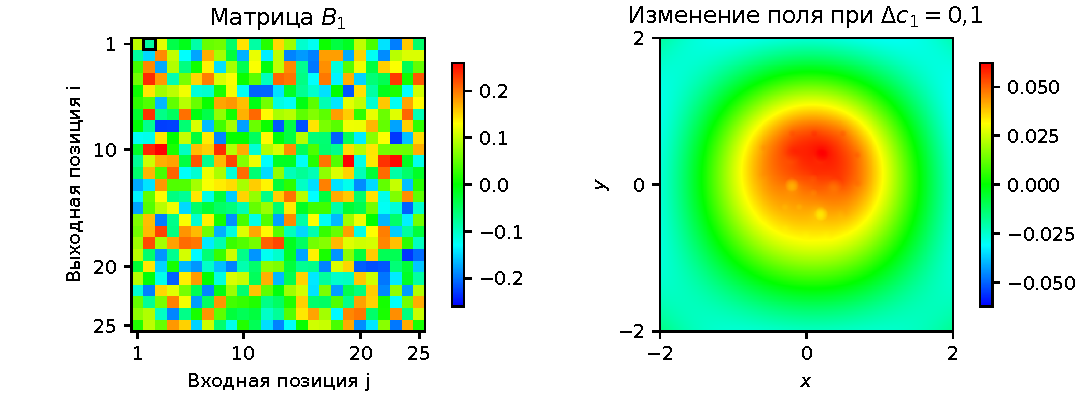
\includegraphics[width=.91\linewidth]{assets/operator_matrices.pdf}
\captionsetup{hypcap=false}\captionof{figure}{Слева оба индекса обозначают позиции
мод в первом блоке сети. Рамкой выделен вес $(B_1)_{1,2}$. Справа показано
изменение прогноза $0{,}1\phi_{1,R}(x)$ в физических координатах на эталонной сетке.
У каждой карты своя шкала с нулём в зелёном.}
\end{center}

